\documentclass[12pt]{article}
\usepackage{geometry}
\geometry{a4paper, margin=1in}
\usepackage{enumitem}
\usepackage{hyperref}
\usepackage{tocloft}
\usepackage{graphicx}
\hypersetup{
    colorlinks=true,
    linkcolor=blue,
    urlcolor=cyan,
}

\title{CS3338 Group 3 Design Specification\\\textbf{Want2Remember}}
\author{}
\date{}

\begin{document}

\maketitle
\thispagestyle{empty}
\newpage

\tableofcontents
\newpage

\section{Snapshot Objectives}
\textbf{Objective:} Our main objective is to develop a product that will support the performance of our user's short-term memory.capabilities.\newline
\subsection{Snapshot 1}
\textbf{Delegation:} Initial feature to be completed: \textbf{Home Page}\newline
\textbf{Dependencies:}
\begin{itemize}
    \item JavaScript
    \item ReactJS
    \item GitHub
    \item JIRA and Agile Development Technology
    \item Firebase
\end{itemize}

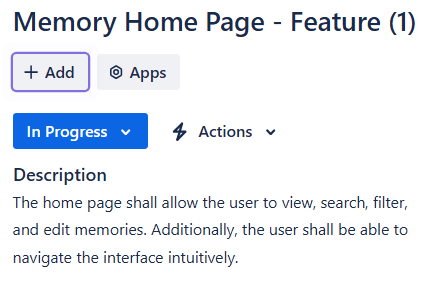
\includegraphics{snapshot1img1.png}\newline
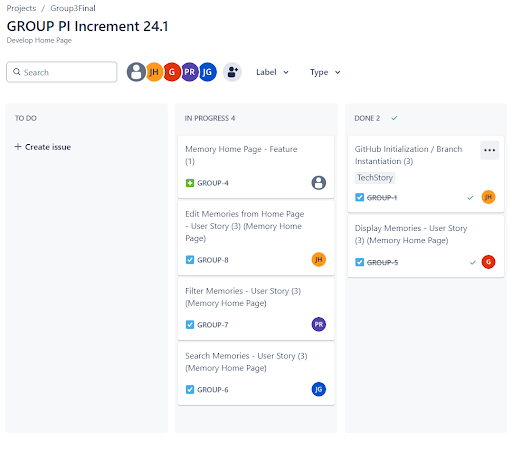
\includegraphics{snapshot1img2.png}
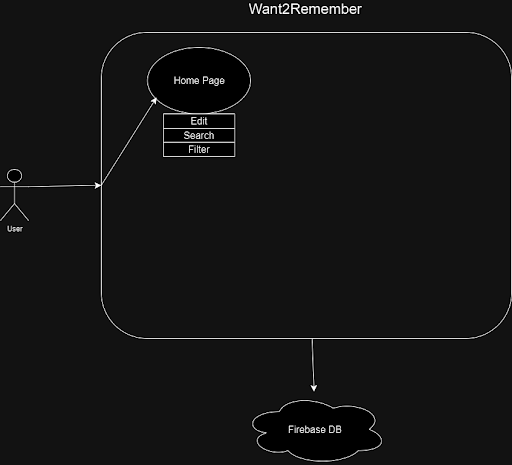
\includegraphics{snapshot1img3.png}
\textbf{Description:}The outer boundary represents the scope of the Want2Remember Product. Within shows different features as bubbles and their associated functionality as a table below. Outside of the boundary are external functionalities. The arrows represent the data flow of the product.


\subsection{Snapshot 2}
\textbf{Objective:} To create a page that will allow users to create memories that can later be accessed from the DB.\newline Dependencies Added :
\begin{itemize}
    \item
     TestRail
\end{itemize}
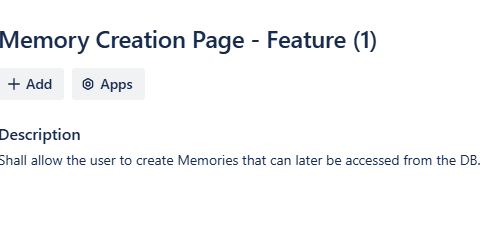
\includegraphics{snapshot2img1.png}
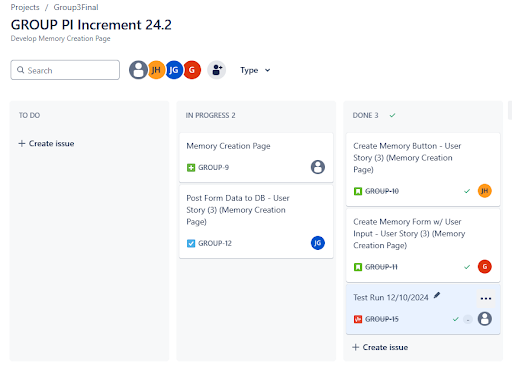
\includegraphics{snapshot2img2.png}
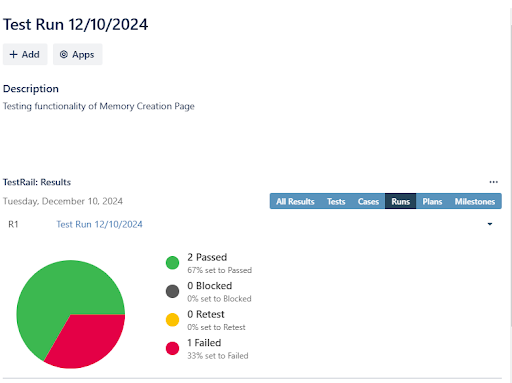
\includegraphics{snapshot2img3.png}
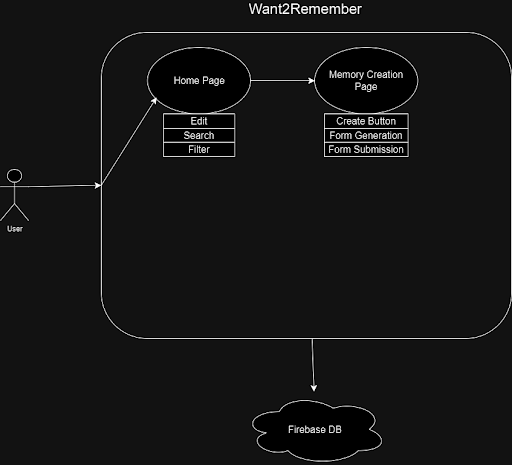
\includegraphics{snapshot2img4.png}

\subsection{Snapshot 3}
\textbf{Objective:} Complete the More Detail Page. \newline
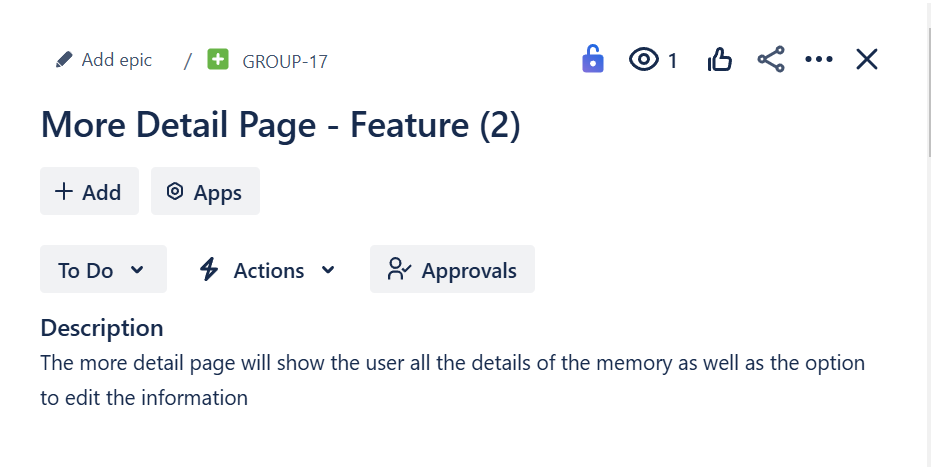
\includegraphics{snapshot3img1.png}
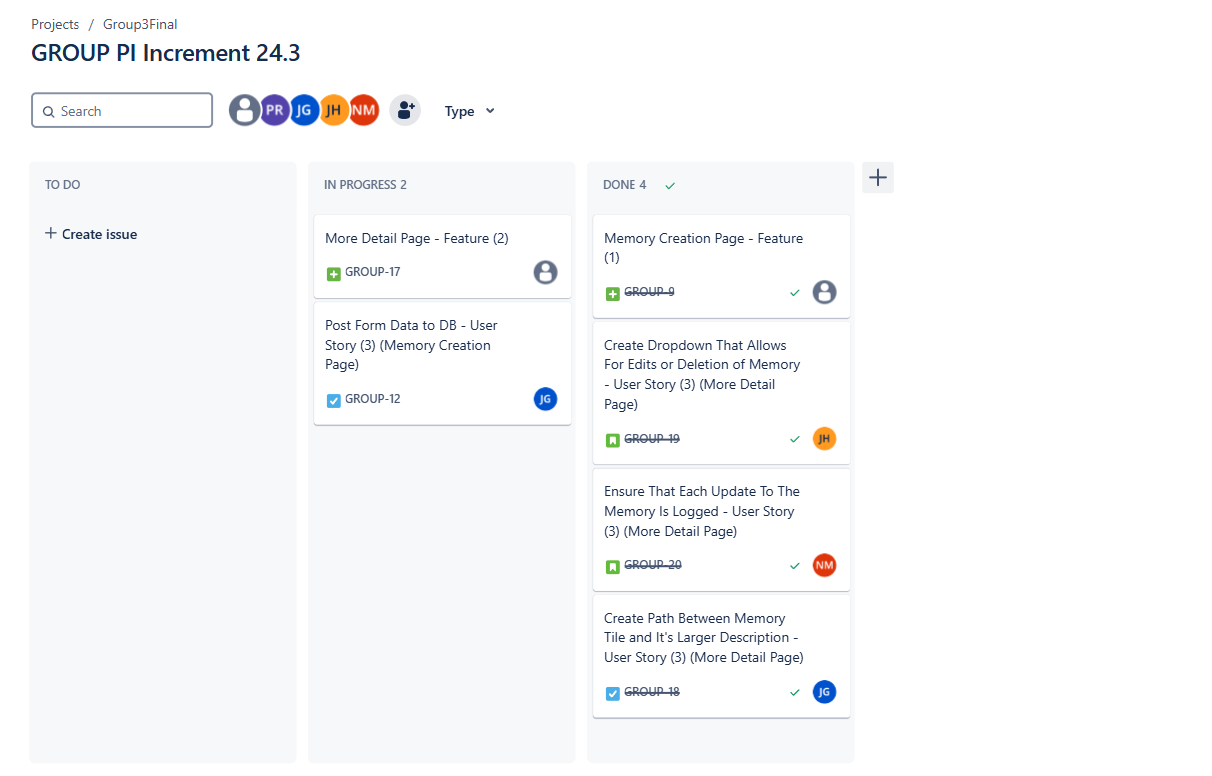
\includegraphics{snapshot3img2.png}\newline
\includegraphics[width=.9\linewidth]{snapshot3img3.png}\newline
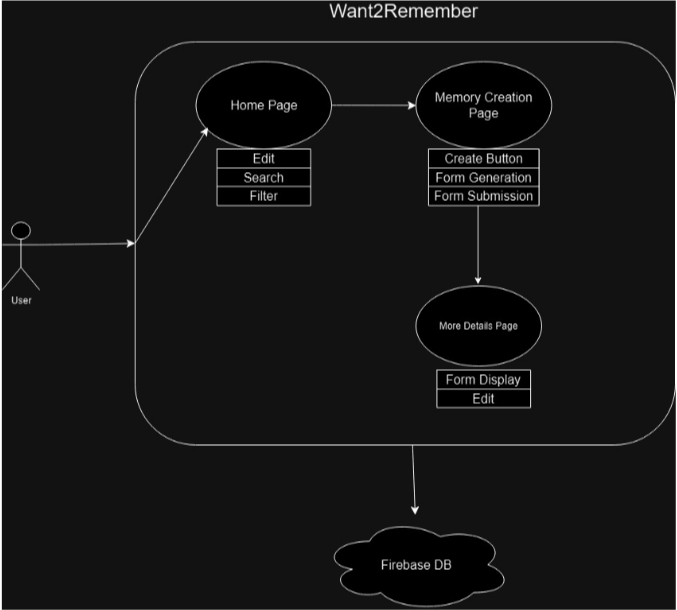
\includegraphics{snapshot3img4.png}

\subsection{Snapshot 4}
\textbf{Objective:} Memory Contact Page\newline
\includegraphics{snapshot4img1.png}\newline
\includegraphics{snapshot4img2.png}\newline
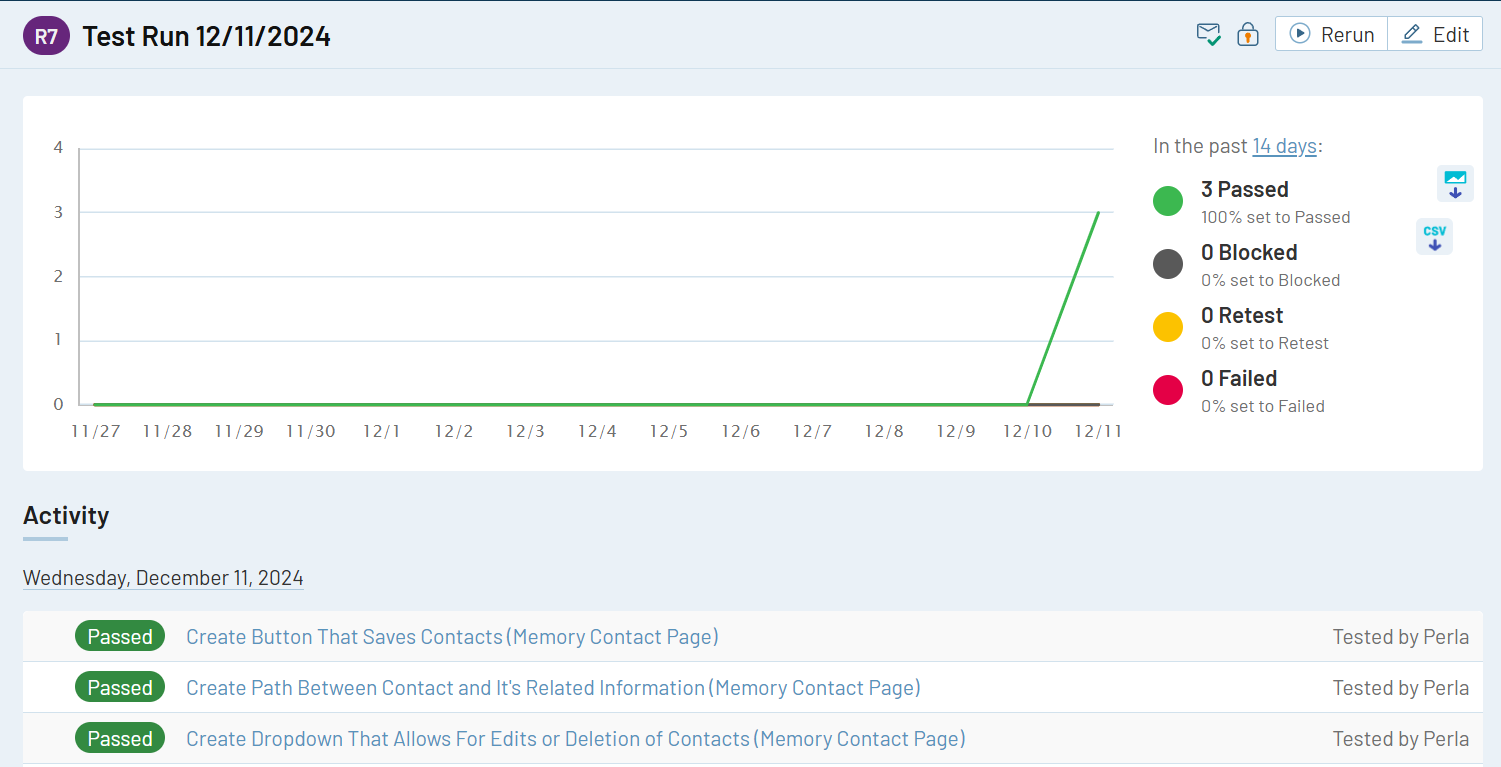
\includegraphics[width=.9\linewidth]{snapshot4img3.png}\newline
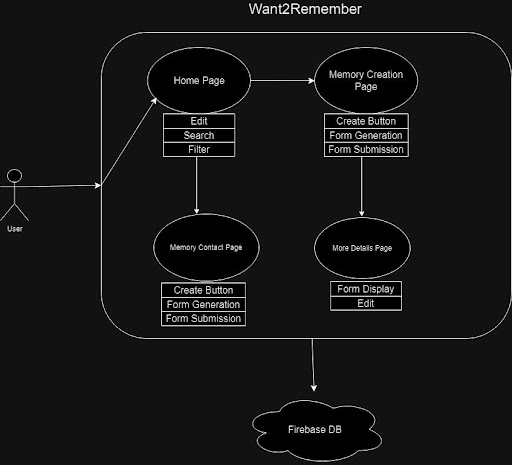
\includegraphics{snapshot4img4.jpg}


\section{Design Breakdown}

\subsection{Home Page}
\textbf{Purpose:}The home page will provide navigation to other pages and a brief overview of created memories.

\textbf{Features:}
\begin{itemize}
    \item List of all memories created by the user, displayed with details like title and date.
    \item Intuitive interface to ensure ease of use for users.
    \item Links to navigate to Memory Creation, More Detail, and Memory Contact pages.
\end{itemize}

\subsection{Memory Creation Page}
\textbf{Purpose:}Allows users to create and save new memories with detailed information.

\textbf{Features:}
\begin{itemize}
    \item Form for memory input, including fields like title, description, tags, and categories.
    \item Firebase integration to store data in a secure backend.
\end{itemize}

\subsection{More Detail Page}
\textbf{Purpose:} The More Detail Page will show the user all the details of the memory as well as the option to edit the information

\textbf{Features:}
\begin{itemize}
    \item Displays all details of a selected memory.
    \item Edit button to allow modifications to the memory’s title, description, or other fields.
    \item Navigation back to the Home Page or other pages after editing.
\end{itemize}

\subsection{Memory Contact Page}
\textbf{Purpose:}The Memory Contact Page will show the user all contacts they have saved

\textbf{Features:}
\begin{itemize}
     \item Displays all saved contacts relevant to the user’s memories.y.
    \item Option to add, edit, or delete contact details.
    \item Links to a detailed contact view for individual contact information.
\end{itemize}

\section{Development Tools}
\begin{itemize}
    \item \textbf{JavaScript and ReactJS:} Used for front-end development.
    \item \textbf{GitHub:} Version control and collaboration.
    \item \textbf{JIRA:} Task tracking and Agile development.
    \item \textbf{Firebase:} Backend as a service for authentication and database management.
\end{itemize}
\section{Future Work}
\begin{itemize}
    \item \textbf{Improve Caregiver Features:} Some of the features that will help caregivers include GPS tracking of supported users and automatic role assignments. Another feature includes allowing the caregiver to remotely control the user’s app to showcase to the care receiver how to perform a specific task.
    \item \textbf{Medication Tracking:} Users will be able to set up reminders for medication and medication administration and save things like proofs of prescriptions.
    \item \textbf{Machine Learning/AI Features:} This can include using AI to improve interactivity with the app or implementing smart reminders that can further support people with cognitive impairments.
\end{itemize}

\end{document}


